\documentclass{article}[]
\usepackage{amsfonts, amssymb, amsmath}
\usepackage{graphicx}
\usepackage{float}
\begin{document}
\title{Gate ST 24.2023}
\author{Rusna Shaikh\\EE22BTECH11048}
\date{}
\maketitle{}
\providecommand{\pr}[1]{\ensuremath{\Pr\left(#1\right)}}
\providecommand{\prt}[2]{\ensuremath{p_{#1}^{\left(#2\right)} }}        % own macro for this question
\providecommand{\qfunc}[1]{\ensuremath{Q\left(#1\right)}}
\providecommand{\sbrak}[1]{\ensuremath{{}\left[#1\right]}}
\providecommand{\lsbrak}[1]{\ensuremath{{}\left[#1\right.}}
\providecommand{\rsbrak}[1]{\ensuremath{{}\left.#1\right]}}
\providecommand{\brak}[1]{\ensuremath{\left(#1\right)}}
\providecommand{\lbrak}[1]{\ensuremath{\left(#1\right.}}
\providecommand{\rbrak}[1]{\ensuremath{\left.#1\right)}}
\providecommand{\cbrak}[1]{\ensuremath{\left\{#1\right\}}}
\providecommand{\lcbrak}[1]{\ensuremath{\left\{#1\right.}}
\providecommand{\rcbrak}[1]{\ensuremath{\left.#1\right\}}}
\newcommand{\sgn}{\mathop{\mathrm{sgn}}}
\providecommand{\abs}[1]{\left\vert#1\right\vert}
\providecommand{\res}[1]{\Res\displaylimits_{#1}} 
\providecommand{\norm}[1]{\left\lVert#1\right\rVert}
%\providecommand{\norm}[1]{\lVert#1\rVert}
\providecommand{\mtx}[1]{\mathbf{#1}}
\providecommand{\mean}[1]{E\left[ #1 \right]}
\providecommand{\cond}[2]{#1\middle|#2}
\providecommand{\fourier}{\overset{\mathcal{F}}{ \rightleftharpoons}}
\newenvironment{amatrix}[1]{%
  \left(\begin{array}{@{}*{#1}{c}|c@{}}
}{%
  \end{array}\right)
}
%\providecommand{\hilbert}{\overset{\mathcal{H}}{ \rightleftharpoons}}
%\providecommand{\system}{\overset{\mathcal{H}}{ \longleftrightarrow}}
	%\newcommand{\solution}[2]{\textbf{Solution:}{#1}}
\newcommand{\solution}{\noindent \textbf{Solution: }}
\newcommand{\cosec}{\,\text{cosec}\,}
\providecommand{\dec}[2]{\ensuremath{\overset{#1}{\underset{#2}{\gtrless}}}}
%\newcommand{\brak}[1]{\ensuremath{\begin{pmatrix}#1\end{pmatrix}}}
\newcommand{\mydet}[1]{\ensuremath{\begin{vmatrix}#1\end{vmatrix}}}
\newcommand{\myaugvec}[2]{\ensuremath{\begin{amatrix}{#1}#2\end{amatrix}}}
\providecommand{\rank}{\text{rank}}
\providecommand{\pr}[1]{\ensuremath{\Pr\left(#1\right)}}
\providecommand{\qfunc}[1]{\ensuremath{Q\left(#1\right)}}
	\newcommand*{\permcomb}[4][0mu]{{{}^{#3}\mkern#1#2_{#4}}}
\newcommand*{\perm}[1][-3mu]{\permcomb[#1]{P}}
\newcommand*{\comb}[1][-1mu]{\permcomb[#1]{C}}
\providecommand{\qfunc}[1]{\ensuremath{Q\left(#1\right)}}
\providecommand{\gauss}[2]{\mathcal{N}\ensuremath{\left(#1,#2\right)}}
\providecommand{\diff}[2]{\ensuremath{\frac{d{#1}}{d{#2}}}}
\providecommand{\myceil}[1]{\left \lceil #1 \right \rceil }
\newcommand\figref{Fig.~\ref}
\newcommand\tabref{Table~\ref}
\newcommand{\sinc}{\,\text{sinc}\,}
\newcommand{\rect}{\,\text{rect}\,}
%%
%	%\newcommand{\solution}[2]{\textbf{Solution:}{#1}}
%\newcommand{\solution}{\noindent \textbf{Solution: }}
%\newcommand{\cosec}{\,\text{cosec}\,}
%\numberwithin{equation}{section}
%\numberwithin{equation}{subsection}
%\numberwithin{problem}{section}
%\numberwithin{definition}{section}
%\makeatletter
%\@addtoreset{figure}{problem}
%\makeatother

%\let\StandardTheFigure\thefigure
\let\vec\mathbf

Q.24 Let $X_1, X_2,...,X_n$ be a random sample of size $n$ from a population having uniform distribution over the interval $\brak{\frac{1}{3},\theta}$, where $\theta>\frac{1}{3}$ is an unknown parameter. If $Y = $ max \{$X_1, X_2,...,X_n$\}, then which one of the following statements is true?
\begin{enumerate}
\item $\brak{\frac{n+1}{n}}\brak{Y-\frac{1}{3}} + \frac{1}{3}$ is an unbiased estimator of $\theta$
\item $\brak{\frac{n}{n+1}}\brak{Y-\frac{1}{3}} + \frac{1}{3}$ is an unbiased estimator of $\theta$
\item $\brak{\frac{n+1}{n}}\brak{Y+\frac{1}{3}} - \frac{1}{3}$ is an unbiased estimator of $\theta$
\item $Y$ is an unbiased estimator of $\theta$
\end{enumerate} 

\solution

Any one of the above expressions is an unbiased estimator of $\theta$ if 
$$E(\text{estimator})=\theta$$

We will first calculate expected value of Y

The PDF of $X_i$ can be expressed as
\begin{align}
p_{X_i}(x)=\frac{1}{\theta-\frac{1}{3}} \text{ , }  \frac{1}{3}<\theta<3
\end{align}

\begin{align}
F_{X_i}(y)&=\int_{\frac{1}{3}}^{y} p_{X_i}(x) dx \\
&=\int_{\frac{1}{3}}^{y} \frac{1}{\theta-\frac{1}{3}} dx \\
&=\frac{y-\frac{1}{3}}{\theta-\frac{1}{3}}
\end{align}

\begin{align}
F_X(y)&=\Pr(X \leq y)\\
&=\Pr(X_1 \leq y, X_2 \leq y,..., X_n \leq y)\\
&=\Pr(X_1 \leq y)\Pr(X_2 \leq y)...\Pr(X_n \leq y)\\
&=\brak{\frac{y-\frac{1}{3}}{\theta-\frac{1}{3}}}^n
\end{align}

\begin{align}
p_X(y)&=\frac{d}{dy} F_X(y) \\
&=\frac{n}{\brak{\theta-\frac{1}{3}}^n} \brak{y-\frac{1}{3}}^n 
\end{align}

\begin{align}
E(Y)&=\int_{\frac{1}{3}}^{\theta} yp_X(y) dy \\ 
&=\int_{\frac{1}{3}}^{\theta} y\frac{n}{\left(\theta-\frac{1}{3}\right)^n} \left(y-\frac{1}{3}\right)^n dy \\ 
&=\frac{n}{\brak{\theta-\frac{1}{3}}^n}\int_{\frac{1}{3}}^{\theta} y\brak{y-\frac{1}{3}}^{n-1} dy \\ 
\text{Let } y-\frac{1}{3}=t\\
\implies y=t+\frac{1}{3} \implies dy=dt \\
\text{Therefore,}\\
E(Y)&=\frac{n}{\brak{\theta-\frac{1}{3}}^n}\int_{0}^{\theta-\frac{1}{3}} \brak{t^n+\frac{t^{n-1}}{3}} dt \\
&=\frac{n}{\brak{\theta-\frac{1}{3}}^n} \brak{\frac{\brak{\theta-\frac{1}{3}}^{n+1}}{n+1} + \frac{\brak{\theta-\frac{1}{3}}^n}{3n}}\\
&=\frac{n}{n+1}\brak{\theta-\frac{1}{3}} + \frac{1}{3}\\
&=\frac{3n\theta + 1}{3(n+1)} \neq \theta
\end{align}

Therefore, fourth option is incorrect.

\begin{enumerate}
\item
{
\begin{align}
E(\brak{\frac{n+1}{n}}\brak{Y-\frac{1}{3}} + \frac{1}{3}) &= \frac{n+1}{n}E(Y)-\frac{n+1}{3n} + \frac{1}{3}\\
&=\frac{3n\theta+1-(n+1)+n}{3n}\\
&=\theta
\end{align}
It is the unbiased estimator of $\theta$.
}
\item
{
Similarly,
\begin{align}
E(\brak{\frac{n}{n+1}}\brak{Y-\frac{1}{3}} + \frac{1}{3})&=\frac{n}{n+1}E(Y) - \frac{n}{3(n+1)} + \frac{1}{3}\\
&=\frac{n(3n\theta+1) - n(n+1) + (n+1)^2}{3(n+1)^2}\\
&=\frac{3n^2+n}{3(n+1)^2} \neq \theta
\end{align}
It is not an unbiased estimator of $\theta$.
}
\item
{
In the same way,
\begin{align}
E(\brak{\frac{n+1}{n}}\brak{Y+\frac{1}{3}} - \frac{1}{3})&=\frac{n+1}{n}E(Y) + \frac{n+1}{3n} - \frac{1}{3}\\
&=\frac{3n\theta+1+n+1-n}{3n}\\
&=\frac{3n\theta+2}{3n} \neq \theta
\end{align}
It is not an unbiased estimator of $\theta$.
}
\end{enumerate}
Hence, the first option is the correct option.

\begin{figure}[H]
\centering
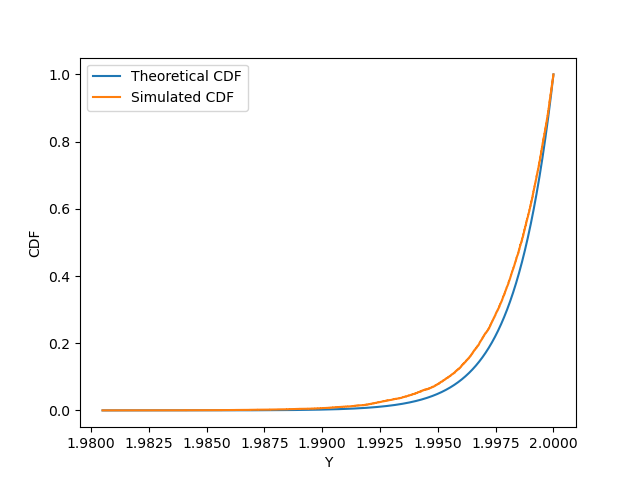
\includegraphics{figs/estimations.png}
\caption{Theoretical and Simulated CDFs}
\label{ST:24.2023}
\end{figure}



Steps for the Simulation using C: 
\begin{enumerate}
\item Include Header Files: Start the C program by includung necessary header files, particularly `<stdio.h>' to perform standard input and output functions.
\item Declare Variables: Declare variables for sample size, number of simulations and $\theta$.
\item Open the file: Use `fopen' to open a file for writing the simulated data. The file is named `estimations.txt'.
\item Simulate data: Use loop to perform multiple simulations. In each iteration, generate random samples, calculate the estimator, and store the estimations in an array.
\item Write data to file: Inside the loop, use `fprintf' to write each estimation to the opened file.
\item Close the file: After all simulations are complete and data is written, close the file using `fclose' to save the data.
\end{enumerate}

Python code for Plotting and Analysis:

Steps: 
\begin{enumerate}
\item Include Required Libraries: In Python code, include libraries like NumPy for data manipulation and Matplotlib for plotting.
\item Load data: Use NumPy to load the data from the file `estimations.txt' into a pyhon array or NumPy array.
\item Define theoretical CDF: Define the function that calculates the theoretical CDF.
\item Sort the data: Sort the loaded data in ascending order.
\item Calculate the empirical CDF: Calculate the empirical CDF for the sorted data by dividing the rank of each value by the total number of data points.
\item Plot the CDFs: Use Matplotlib to create a plot that compares the theoretical and simulated CDFs.
\end{enumerate}
\end{document}
